% ----------------------------------------------------
% Recommendations
% ----------------------------------------------------
\documentclass[class=report,11pt,crop=false]{standalone}
% Page geometry
\usepackage[a4paper,margin=20mm,top=25mm,bottom=25mm]{geometry}

% Font choice
\usepackage{lmodern}

\usepackage{lipsum}

% Use IEEE bibliography style
\bibliographystyle{IEEEtran}

% Line spacing
\usepackage{setspace}
\setstretch{1.20}

% Ensure UTF8 encoding
\usepackage[utf8]{inputenc}

% Language standard (not too important)
\usepackage[english]{babel}

% Skip a line in between paragraphs
\usepackage{parskip}

% For the creation of dummy text
\usepackage{blindtext}

% Math
\usepackage{amsmath}

% Header & Footer stuff
\usepackage{fancyhdr}
\pagestyle{fancy}
\fancyhead{}
\fancyhead[R]{\nouppercase{\rightmark}}
\fancyfoot{}
\fancyfoot[C]{\thepage}
\renewcommand{\headrulewidth}{0.0pt}
\renewcommand{\footrulewidth}{0.0pt}
\setlength{\headheight}{13.6pt}

% Epigraphs
\usepackage{epigraph}
\setlength\epigraphrule{0pt}
\setlength{\epigraphwidth}{0.65\textwidth}

% Colour
\usepackage{color}
\usepackage[usenames,dvipsnames]{xcolor}

% Hyperlinks & References
\usepackage{hyperref}
\definecolor{linkColour}{RGB}{77,71,179}
\hypersetup{
    colorlinks=true,
    linkcolor=linkColour,
    filecolor=linkColour,
    urlcolor=linkColour,
    citecolor=linkColour,
}
\urlstyle{same}

% Automatically correct front-side quotes
\usepackage[autostyle=false, style=ukenglish]{csquotes}
\MakeOuterQuote{"}

% Graphics
\usepackage{graphicx}
\graphicspath{{Images/}{../Images/}}
\usepackage{makecell}
\usepackage{transparent}

% SI units
\usepackage{siunitx}

% Microtype goodness
\usepackage{microtype}

% Listings
\usepackage[T1]{fontenc}
\usepackage{listings}
\usepackage[scaled=0.8]{DejaVuSansMono}

% Custom colours for listings
\definecolor{backgroundColour}{RGB}{250,250,250}
\definecolor{commentColour}{RGB}{73, 175, 102}
\definecolor{identifierColour}{RGB}{196, 19, 66}
\definecolor{stringColour}{RGB}{252, 156, 30}
\definecolor{keywordColour}{RGB}{50, 38, 224}
\definecolor{lineNumbersColour}{RGB}{127,127,127}
\lstset{
  language=Matlab,
  captionpos=b,
  aboveskip=15pt,belowskip=10pt,
  backgroundcolor=\color{backgroundColour},
  basicstyle=\ttfamily,%\footnotesize,        % the size of the fonts that are used for the code
  breakatwhitespace=false,         % sets if automatic breaks should only happen at whitespace
  breaklines=true,                 % sets automatic line breaking
  postbreak=\mbox{\textcolor{red}{$\hookrightarrow$}\space},
  commentstyle=\color{commentColour},    % comment style
  identifierstyle=\color{identifierColour},
  stringstyle=\color{stringColour},
   keywordstyle=\color{keywordColour},       % keyword style
  %escapeinside={\%*}{*)},          % if you want to add LaTeX within your code
  extendedchars=true,              % lets you use non-ASCII characters; for 8-bits encodings only, does not work with UTF-8
  frame=single,	                   % adds a frame around the code
  keepspaces=true,                 % keeps spaces in text, useful for keeping indentation of code (possibly needs columns=flexible)
  morekeywords={*,...},            % if you want to add more keywords to the set
  numbers=left,                    % where to put the line-numbers; possible values are (none, left, right)
  numbersep=5pt,                   % how far the line-numbers are from the code
  numberstyle=\tiny\color{lineNumbersColour}, % the style that is used for the line-numbers
  rulecolor=\color{black},         % if not set, the frame-color may be changed on line-breaks within not-black text (e.g. comments (green here))
  showspaces=false,                % show spaces everywhere adding particular underscores; it overrides 'showstringspaces'
  showstringspaces=false,          % underline spaces within strings only
  showtabs=false,                  % show tabs within strings adding particular underscores
  stepnumber=1,                    % the step between two line-numbers. If it's 1, each line will be numbered
  tabsize=2,	                   % sets default tabsize to 2 spaces
  %title=\lstname                   % show the filename of files included with \lstinputlisting; also try caption instead of title
}

% Caption stuff
\usepackage[hypcap=true, justification=centering]{caption}
\usepackage{subcaption}

% Glossary package
% \usepackage[acronym]{glossaries}
\usepackage{glossaries-extra}
\setabbreviationstyle[acronym]{long-short}

% For Proofs & Theorems
\usepackage{amsthm}

% Maths symbols
\usepackage{amssymb}
\usepackage{mathrsfs}
\usepackage{mathtools}

% For algorithms
\usepackage[]{algorithm2e}

% Spacing stuff
\setlength{\abovecaptionskip}{5pt plus 3pt minus 2pt}
\setlength{\belowcaptionskip}{5pt plus 3pt minus 2pt}
\setlength{\textfloatsep}{10pt plus 3pt minus 2pt}
\setlength{\intextsep}{15pt plus 3pt minus 2pt}

% For aligning footnotes at bottom of page, instead of hugging text
\usepackage[bottom]{footmisc}

% Add LoF, Bib, etc. to ToC
\usepackage[nottoc]{tocbibind}

% SI
\usepackage{siunitx}

% For removing some whitespace in Chapter headings etc
\usepackage{etoolbox}
\makeatletter
\patchcmd{\@makechapterhead}{\vspace*{50\p@}}{\vspace*{-10pt}}{}{}%
\patchcmd{\@makeschapterhead}{\vspace*{50\p@}}{\vspace*{-10pt}}{}{}%
\makeatother
\makenoidxglossaries

\newacronym{radar}{RADAR}{Radio Detection and Ranging}

\begin{document}
	% ----------------------------------------------------
	\chapter{User Interface \label{ch:user-interface}}
	
	\vspace{0.5cm}
	% ----------------------------------------------------
	
	\section{Introduction}
	This chapter deals with the user interface of the system. The user interface is how the client will be able to make use of the system.
	
	\section{Requirements}
	
		\subsection{User Requirements}
		\begin{enumerate}
			\item Display weight data on app.
			\item App must have interface for manual data.
			\item Other data should be automated (time, location).
			\item Data must be saved to a spreadsheet. It should have the following fields: FID, Date, Time, ID, Ring type, Sex, Mass, Day status, Day status, Day, Weekday, Term, Name, Weight Session, Location, Notes, People Count 1, People Count 2.
			
		\end{enumerate}
		
		\subsection{Functional Requirements}
		\begin{enumerate}
			\item Establish connection between smart scale (Arduino) and phone (via Bluetooth or Wi-Fi) 
			\item The GUI should have a text box to input the bird's ID.
			\item A CSV file needs to be created where the data will be written.
		\end{enumerate}
			
			
		
	
		
	
	\section{Design Choices}
		
	
		\subsection{Sending readings}
		There are several technologies to transmit data such as: Wi-Fi, and Bluetooth. 
		Wi-Fi has the benefit of conneting to the internet. It requires minimal effort on the user's end if they are already connected to the internet . However, internet access is not feasible as weighing sessions span outside of \textit{eduroam} coverage.
		Bluetooth is more power effecient, which is important because the scale must be portable. 
		A comparative graph of power usage from Eridani et al. \cite{comparitiveEspnow} is shown below in figure \ref{fig:power-usage}.
		
		\begin{figure}[h!]
			\centering
			\includegraphics[scale=0.7]{"Figures/Power usage"}
			\caption{Power Usage Graph}
			\label{fig:power-usage}
		\end{figure}
		
		In addition, Bluetooth's speed is sufficient because only several bytes of data are being transmitted at a time.
		There are two types of Bluetooth: Bluetooth Classic and Bluetooth Low Energy (BLE). BLE is a newer technology that is even more power efficient than Bluetooth Classic; therefore, Bluetooth Low Energy was chosen.
		
		
		%\subsection{Receiving readings}
		
		\subsection{Graphical User Interface}
		A mobile app needed to be developed to receive and record the data. The client uses an Android device; therefore, an the app was developed for Android devices. The official native programming language is Java. Kotlin is a newer language, that Google will be giving more support to than Java, going forward \cite{kotlin}. In addition, Kotlin has more concise and safer code. It has less boilerplate and it has many language features to avoid common programming mistakes, such as null safety \cite{kotlin}.
		
		For these reasons Kotlin was chosen since it would mean this program would be easier to maintain for newer Android devices in the future and it would be less error prone.
		
		Its UI App Development Toolkit, Jetpack Compose, was used to develop the GUI for the app. This was used instead of XML (Extended Markup Language), since it is more concise than XML, and is officially supported by Google.
			
		
		\subsection{Saving data}
		The data is required to be viewed in a spreadsheet form. The simplest format that can be read in a spread sheet is the CSV (Comma Separated Values) format. The other common option is the Excel Workbook format for Microsoft Excel. This format is more complicated and unnecessary, since only text values are being saved.
		
	
	\section{Subsystem Design}
		
		\begin{figure}[h!]
			\centering
			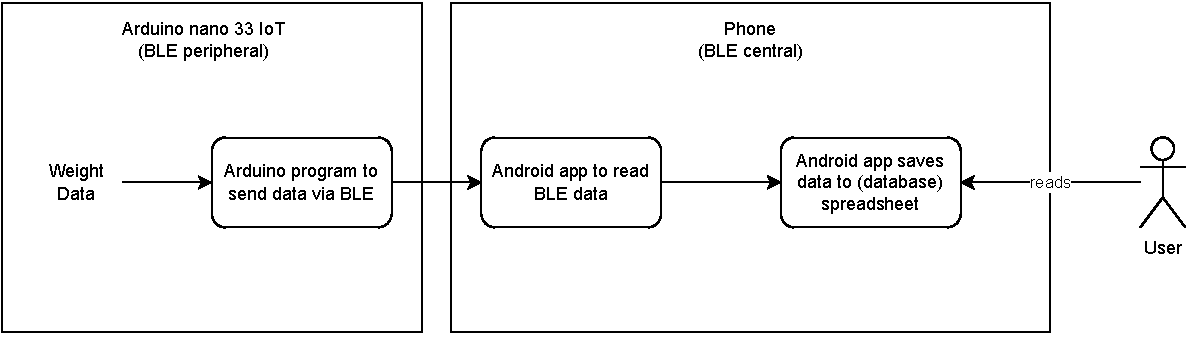
\includegraphics[width=0.9\linewidth]{Figures/Starling data block diagram.pdf}
			\caption{Block diagram of subsystem}
		\end{figure}
		
		This subsystem exists in two environments: the Arduino, and the mobile device. The Arduino needs to be programmed to send the weight readings to the mobile device. A mobile app needs to be developed to receive the weight readings. The app needs to provide a GUI that allows the user to input the bird's ID. The app should save the data to a spreadsheet for the user to view.
		
	
		\subsection{Sending data}
		
			BLE works differently to Bluetooth Classic. Bluetooth Classic is based on an asynchronous serial connection. BLE, on the other hand, works like a community bulletin board \cite{ble}. The peripheral device posts data for central devices to read \cite{ble}.This model is shown below in figure \ref{fig:ble-bulletin-board-model}.
			
			\begin{figure}[h!]
				\centering
				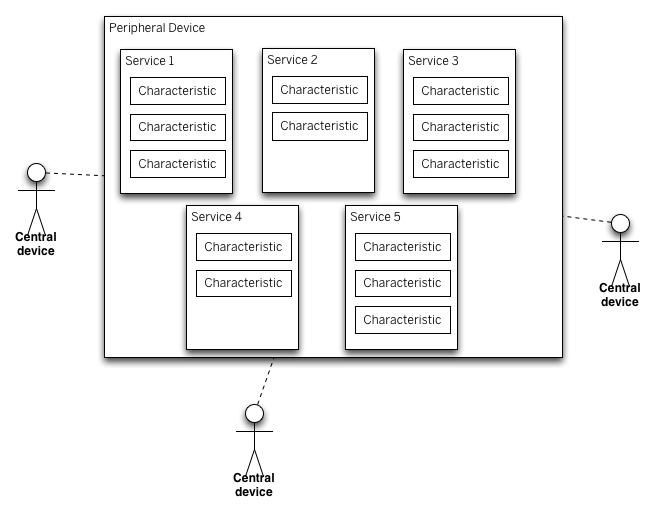
\includegraphics[scale=0.5]{Figures/ble-bulletin-board-model}
				\caption{BLE Bulletin Board Model \cite{ble}}
				\label{fig:ble-bulletin-board-model}
			\end{figure}
			
			The information presented by the peripheral device is structured as services, which are subdivided into characteristics \cite{ble}. BLE includes a mechanism known as notify. This notifies central devices when the data changes.
			
			A program was developed and uploaded to the Arduino. This program, \href{https://github.com/karanimaan/EEE4113F-Project--Group-26/blob/main/send_data/send_data.ino}{send\_data.ino}, can be found under the \textit{send\_data} folder in the project repository.
			Firstly, in the setup function, the BLE name of the device is set to "Arduino Nano 33 IoT".
			Then, a custom service is advertised and a characteristic is added to the service.
			In an infinite loop, the program checks if a central device is connected. If there is, then the weight value is converted to a string and written in to the \textit{weight} characteristic. The connected central device would then be able to read the \textit{weight} reading as a string.
			
		%\subsection{Reading data}
		
		
		\subsection{Mobile app}
		
			
			https://github.com/karanimaan/EEE4113F-Project--Group-26/tree/main/Mobile%20App
			
			The Graphical User Interface (GUI) is responsible for displaying the live reading coming from the Arduino, and allowing the user to capture that reading and input the bird ID. The GUI also needs a save button to save the data to a file, so that the user can view the data in a spreadsheet.
			The prototype of the GUI is shown below in figure \ref{fig:gui-prototype}.
			
			\begin{figure}[h!]
				\centering
				\includegraphics[scale=1]{"Figures/GUI prototype"}
				\caption{GUI prototype}
				\label{fig:gui-prototype}
			\end{figure}
		
			Firstly, a column (vertical layout) is created. Within it, the components are created. A screenshot of the GUI on startup is shown below in figure \ref{label}.
		
		
		
		\subsection{Saving data}
			
			
			\begin{figure}
				\centering
				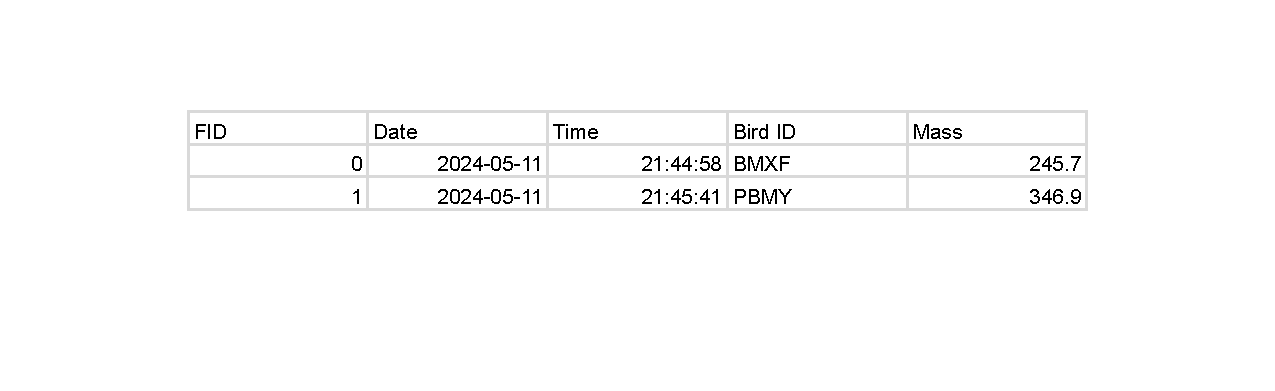
\includegraphics[width=\linewidth]{Figures/exported_data}
				\caption{}
				\label{fig:exporteddata}
			\end{figure}
		
		The spreadsheet should have the following fields: FID, Date, Time, ID, Ring type, Sex, Mass, Day status, Day status, Day (of week), Weekday, Term, Name, Weighing Session, Location, Notes, People Count 1, People Count 2.
		
		FID - pk
		Date, Time, Day, Weekday, Weighing Session, Location - Kotlin
		ID, Day status, Name, Notes, People Count 1, People Count 2 - user
		Ring type, Sex - BirdID table
		Mass - Arduino
		Term - Terms table
		
	
	%\section{Final Design}
	
	%\section{Testing}
	\section{Acceptance Test Procedure}
	Testing was done on a Samsung S9 phone running Android 10.
	\section{Unit Testing}
		
		\subsection{Sending data}
		For the purpose of unit testing, the weight value was hard-coded to $346.2$.
		\textit{LightBlue}, a mobile app, was used to test the Arduino sending data. Screenshots of the process are shown below in figure \ref{fig:screenshots-of-testing-ble-posting}.
		
		\begin{figure}[h!]
			\centering
			\includegraphics[width=1.2\linewidth]{"Figures/Screenshots of testing BLE posting"}
			\caption{Testing the Arduino sending data}
			\label{fig:screenshots-of-testing-ble-posting}
		\end{figure}
	
		On the homepage, a list of devices is displayed. The device "Arduino Nano 33 IoT" was connected to. The service was selected and the characteristic was read. The data format "UTF-8 String" was selected, and the weight reading was displayed. This reading corresponded with the hard-coded value in \href{https://github.com/karanimaan/EEE4113F-Project--Group-26/blob/main/send_data/send_data.ino}{send\_data.ino}.

	
	\subsection{User Acceptance Testing}
	
	\section{Conclusion}
	
	% ----------------------------------------------------
	\ifstandalone
	\bibliography{../Bibliography/References.bib}
	\printnoidxglossary[type=\acronymtype,nonumberlist]
	\fi
\end{document}
% ----------------------------------------------------